\chapter{Facade}

In this chapter, the terminal building facade is going to be designed. To do so, different aspects and issues have been accounted such as: building location, solar incidence, among other factors.

Apart from the aspects that mainly constitute the facade, all the facade-integrated elements will be decided such as doors, windows and access gates. 

	\section{Front, back and dock facades}
		\subsection{Requirements and adopted solution}
		
It has been decided to use a glass facade for several reasons. Apart from current trends and fashions, the reasons why it has been chosen are:
\begin{itemize}
\item \textbf{Providing a calming feeling to the passengers}: glass facades allow to see through them, enabling the passengers to see the take-offs and landings, making them lose fear and providing a relaxing feeling.
\item \textbf{Increasing luminosity}: the glass facade increases luminosity naturally lighting the interior of the building during day-time hours. Sometimes, excessive sun incidence can be a disturbing factor that has to be studied and managed properly.
\item \textbf{Providing a spacious enclosure}: the usage of glass facades increases the spacious feeling, being favorable for passengers and employees and thus, avoiding cramped enclosures.
\item \textbf{Aesthetic reasons}: glass facades are modern and provide a beautiful innovative aspect from inside and outside. Furthermore, glass can be highly customizable (opacity, brightness, reflective...) allowing multiple design solutions.
\end{itemize}

The usage of glass facades is constrained by some rules that have to be fulfiled:
\begin{itemize}
\item \textbf{Safety}: in order to avoid that glass breaks or falls apart, it must be used laminated glass (sheet glass). This kind of glass, additionally offers a high protection against UV rays, filtering up to 99\% of them.
\item \textbf{Thermal insulation}: since the facade is an exterior element, it is important to account the thermal insulation. It is highly recommended to use double layered glazing to avoid heat loss, reduce heating consumption and increase comfort.
\item \textbf{Acoustic insulation}: greater or lesser thicknesses or camera widths (in double layered glazing) are to be defined to improve acoustic attenuation.
\item \textbf{Mechanical issues}: depending upon the loads and solicitations, the thicknesses will be greater or lesser.
\end{itemize}

Glass facades present several typologies. In order to justify why it has been chosen one or another, the main four types are going to be presented next:
\begin{itemize}
\item \textbf{Curtain wall}: this system is used in small-medium magnitude. Glass is installed in front of slabs, and it provides a complete closing, giving a modernity aspect.
\item \textbf{Ventilated facade}: glazing system in which a double skin is applied on a curtain wall. 
\item \textbf{Windows closure}: this system is instaled between slabs. It allows to obtain a quick closing of closures, since each level is independent from the others. It is not necessary using firewalls between slabs, because there is no contact point between two closures.
\item \textbf{Spider system}: in this system, the support is provided by stabilizing connectors such as tensioners, glass ribs or steel pillars, that are adhered to the glass surface by means of structural fittings called "spiders".
\end{itemize}

	\begin{figure}[ht!]
	\centering
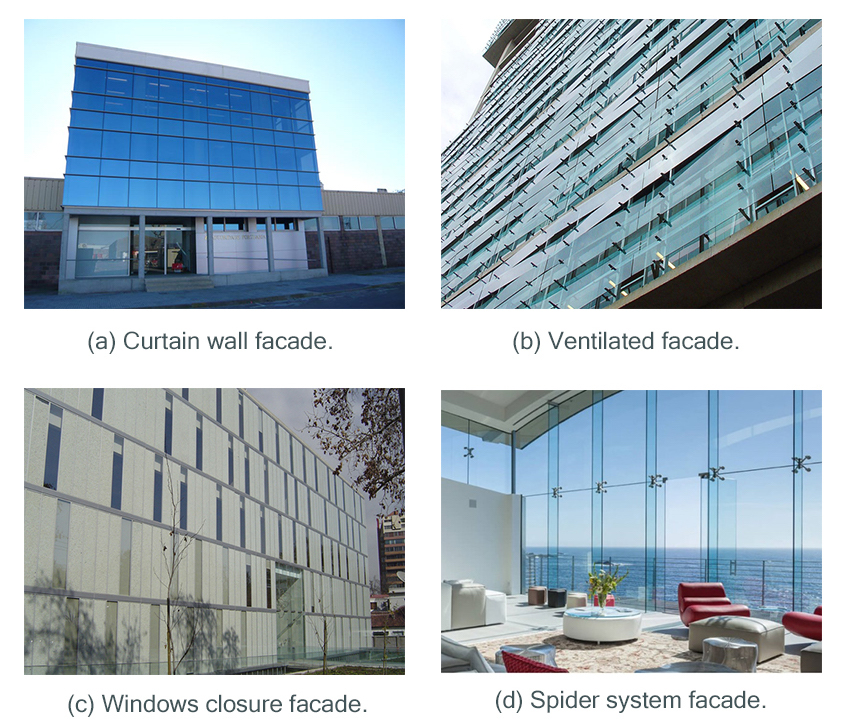
\includegraphics[width=11cm]{./images/Facade/facades}
\caption{Glass facades typologies.}
\end{figure}

Due to the building complexity and the beautiful finishing design, it has been chosen to use a spider system facade. Within this type of facades, there are three different types depending upon the structural fittings that are used: glass ribs, steel pillars or tensioners.

	\begin{figure}[ht!]
	\centering
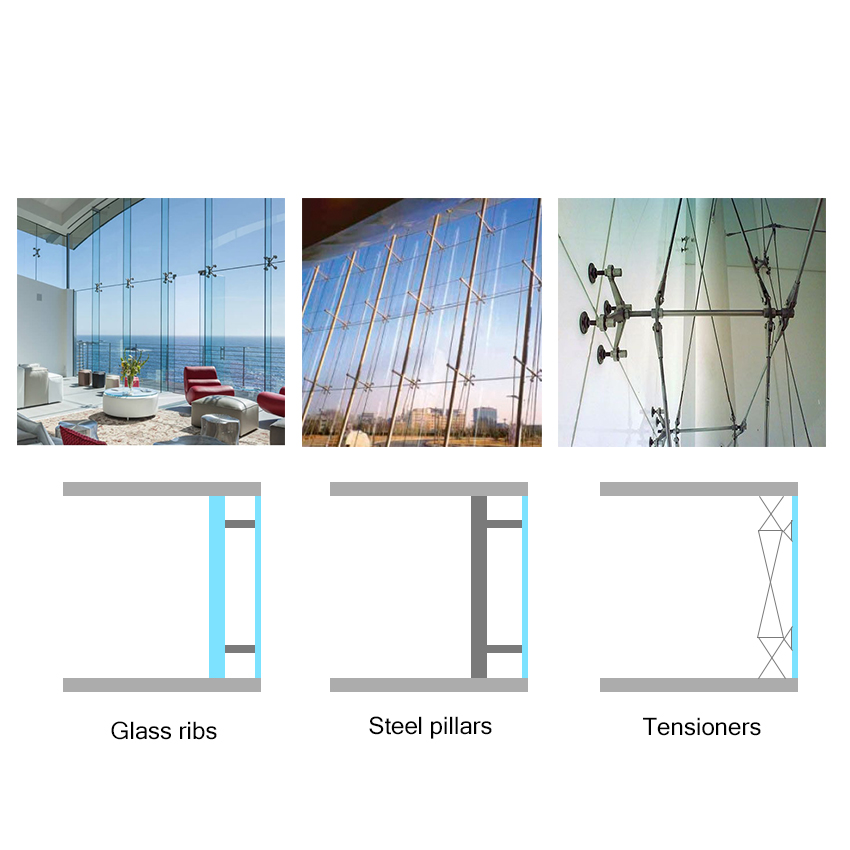
\includegraphics[width=11cm]{./images/Facade/spiders}
\caption{Spider glass system typologies.}
\end{figure}

According to the building characteristics, it has been decided that the spider glass fittings will be steel pillars. The other systems would be too expensive given the dimensions of the building and would become the structure much complex.



		\subsection{Glass}
	The glass to be used is in charge of the SunGuard company. This company recommended to use the Guardian SunGuard Extra Selective SNX 60 glass. It is one of the best products of solar control glass avilable in the current industry.
	
	The SNX 60 has an attractive, uniform, neutral and transparent appearance, regardless the angle of vision. The internal color reflexion has been optimized, allowing a more neutral color tone when it is seen from the inner part of the building. 
	
	This glass, allows the incidence of 60\% of neutral light and only 29\% of solar heat. It is leader in the market for being one of the products with higher selectivity (ratio between light transmission and solar factor). SNX 60 is available in annealing version (recocido) or temperable. Below, one can find a table with the main characteristics of the selected glass:
	
\begin{figure}[ht!]
\centering
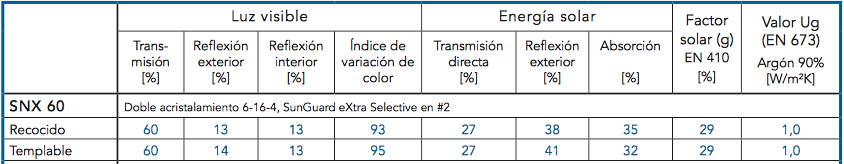
\includegraphics[width=15cm]{./images/Facade/performances}
\caption{Selected glass characteristics (SNX 60).}
\end{figure}

For illustrative purposes, the glass chosen would look as follows in the building:

\begin{figure}[ht!]
\centering
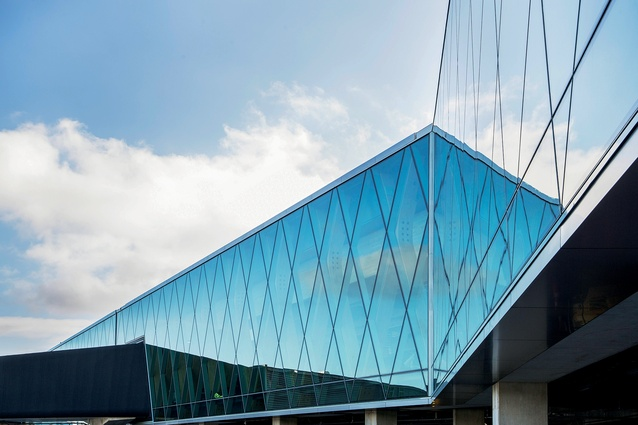
\includegraphics[width=13cm]{./images/Facade/snx60}
\caption{View of a building made of SNX 60.}
\end{figure}

	
	
		\subsection{Spider system with steel pillars}
	The Spider system has been contracted to the German GLASSCON company. They offer all the fittings system for anchoring the glass. The chosen solution has been: Steel supporting solution type "GL/SSS". In this case, only steel pillars would be used, tensioners are not necessary.
	
	\begin{figure}[ht!]
\centering
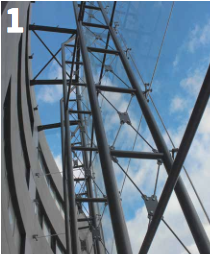
\includegraphics[width=6cm]{./images/Facade/steel}
\caption{Steel supporting solution type "GL/SSS" (GLASSCON).}
\end{figure}
	
		\subsection{Steel and concrete mixed columns}
	Mixed columns are a combination of concrete columns and steel columns, joining advantages from both types of columns. Mixed columns have a greater ductility than purely concrete ones; also, fittings and unions can be built using steel construction techniques. The concrete filling not only provides a greater capacity for supporting loads but also increase the fire resistance.
	
	Different profiles are used for mixed columns. It has been decided to use tubular columns for aesthetical reasons and for the following reasons:
	
\begin{itemize}
\item Concrete filling provides greater stiffness and greater ability of supporting loads in tubular columns. Therefore, aesthetic and thin columns can support large loads without increasing external dimensions.
\item Tubular design is useful for concrete framing and reinforcement.
\item No necessary extra equipment is needed for concrete filling in the tubular design rather than the equipment used in usual concrete works.
\end{itemize}
	
		\begin{figure}[ht!]
\centering
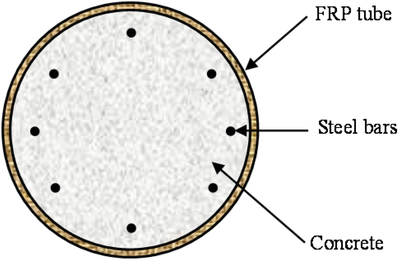
\includegraphics[width=5cm]{./images/Facade/columns}
\caption{Mixed steel and concrete tubular column.}
\end{figure}

In-situ concrete will be provided by the company PT Hume Concrete Indonesia, located a few miles away from the airport location. Tubular steel pillars will be provided by another Indonesian company called Mittal Steel Company.

The columns will be used for supporting the building cover and will have a thickness (diameter) defined by the the structural design team.
	
	
	\section{Secondary areas facade}
		\subsection{Facade (prefabricated concrete)}
	The secondary areas facades of the building, which do not have any aesthetical requirement (since it is where the ABHS (SATE) system, offices and handling dependencies will be allocated) are decided not to be made of glass. 
	
	Several necessities need to be fulfiled, for instance, privacity of the offices but always trying to search for an attractive appearance for the people who will work there. 
	
	For this reason and also for its insulation properties, prefabricated concrete has been decided for closures in the lateral facade including elements such as doors, gates and windows where required.
	
	This material is based on large concrete panels formed in the factory, for this reason, its shapes and dimensions are standardized. The option of providing thermal insulation is available and they can be used either in vertical or horizontal orientation. Another advantage is that they do not need surface finishings since these are included in the forming, as a consequence are aesthetically attractive. The biggest disadvantage is that the structures are heavy and they need a good base structure to make the anchorage.
	
	Other advantages of this structure are: high resistance, clean work, high availability, high durability, excellent fire resistance properties, relatively low price with respect to traditional facades.
	
	The panels are made of architectonic concrete, namely, they are steel-armed concrete. Variable dimensions, thicknesses (from 8cm) and weights are available. These panels have the following features:
	\begin{itemize}
	\item Supporting structures (they are part of the building structure transmitting mechanical stresses to the ground or foundation.
	\item Preformed multilayer with thermal insulation. The insulation material that they contain is expanded polystyrene.
	\end{itemize}

The companies offer prefabricated panels, with a special design to include windows or doors inside.

The company that will provide these prefabricated concrete panels will be Hormipresa S.A., that is leader in its sector having carried out a wide range of projects of all kinds.

Next, the dimensions, properties and features of the slabs (panels) to be instaled are presented:

\begin{table}[ht!]
\centering
\begin{tabular}{|c|c|c|c|c|}
\hline
\vtop{\hbox{\strut Weight} \hbox{\strut [kN/$\mathrm{m^2}$]}} & \vtop{\hbox{\strut Length (L)} \hbox{\strut [m]}} & \vtop{\hbox{\strut Thermal ins.}  \hbox{\strut [kcal/h C $\mathrm{m^2}$]}} & \vtop{\hbox{\strut  Acoustic ins.}  \hbox{\strut [dbA]}} & \vtop{\hbox{\strut Fire resistance} \hbox{\strut [Ei-min]}}\\
\hline
4.00 & 12 & 0.43 & 53.5 & 120\\
\hline
\end{tabular}
\caption{Properties and features of the instaled panels.}
\end{table}

The rectangular slabs will have the following dimensions:
\begin{itemize}
\item Longitude (L): 12 m
\item Longitude (w): 3 m
\item Thickness (e): 2 m
\end{itemize}

Nevertheless, a set of slabs of specific measures will be ordered for areas where the design needs a different kind of measures rather than the standard ones. 

Another issue to be defined is the surface finishing that the lateral facade will have.

	\begin{figure}[ht!]
	\centering
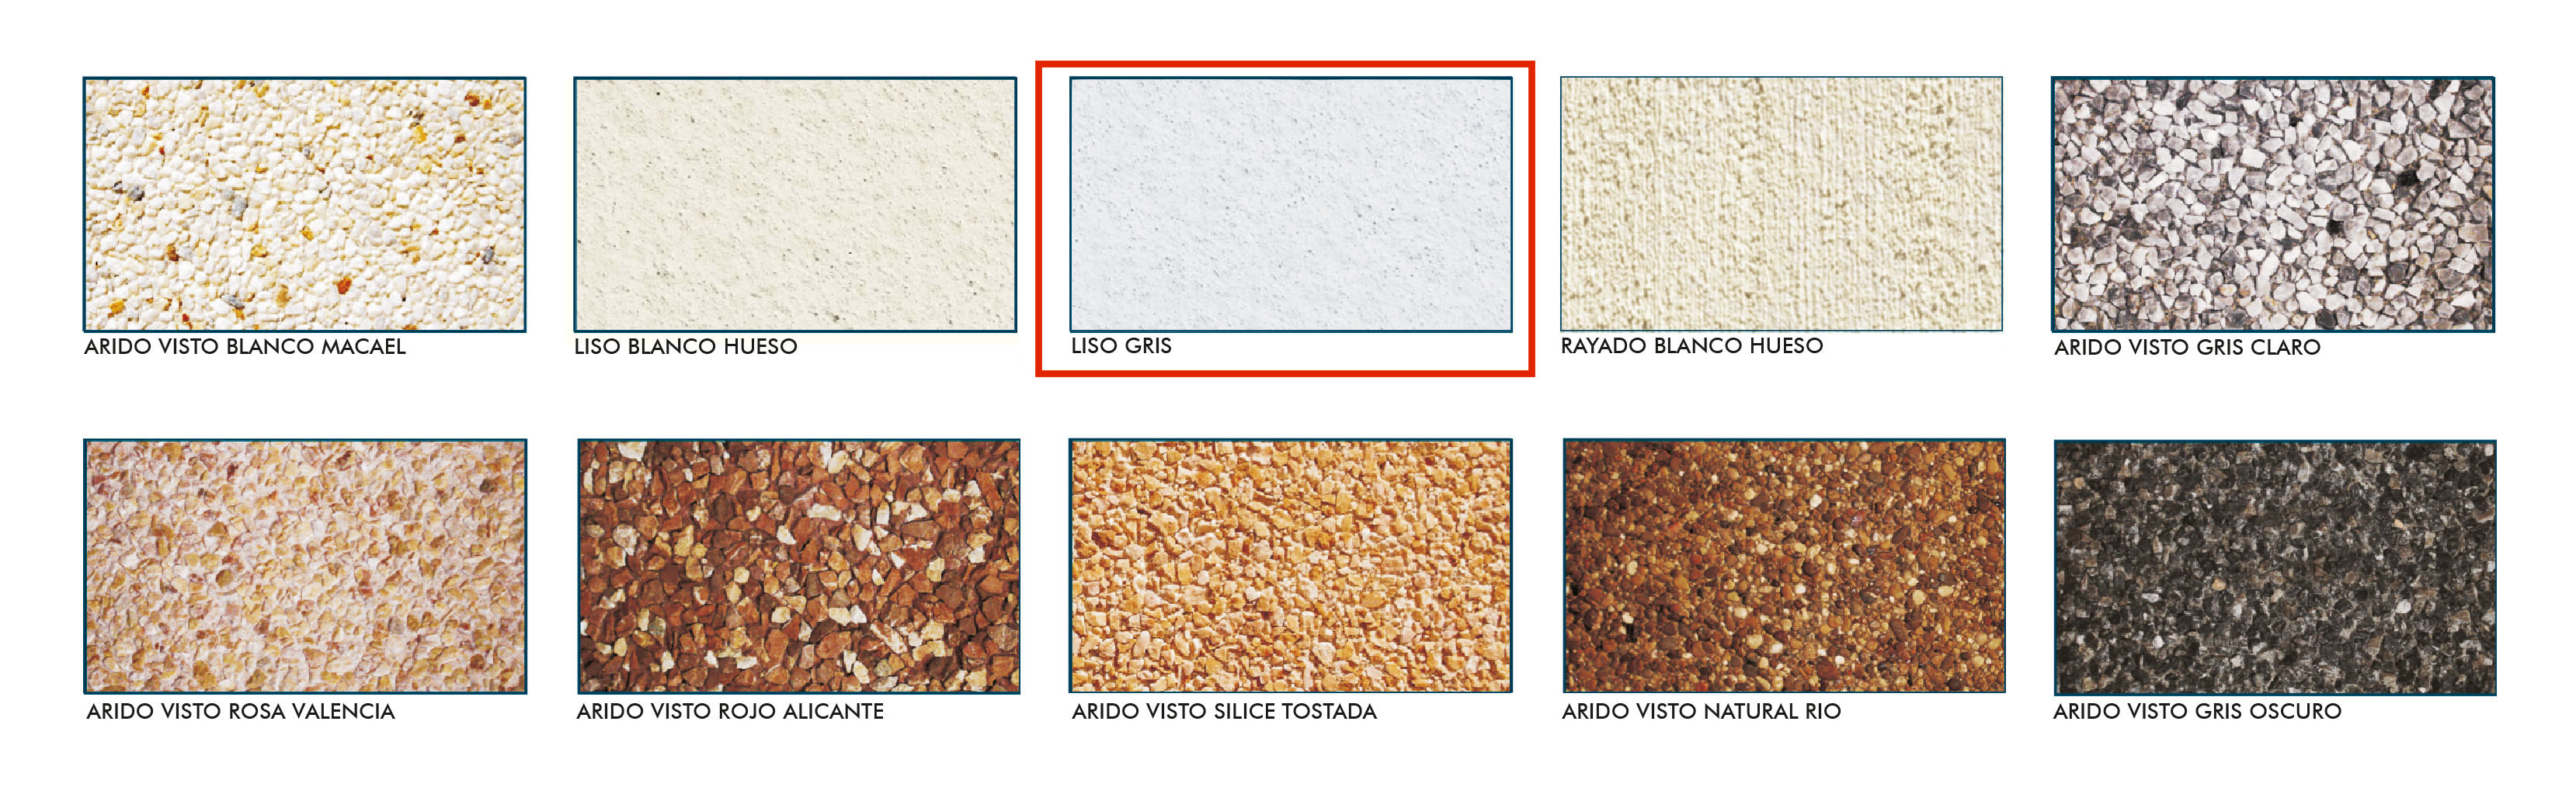
\includegraphics[width=13cm]{./images/Facade/finishing}
\caption{Surface finishing catalogue.}
\end{figure}

The selection has been the smooth gray color, from the catalogue above. Within this possibilities, and taking into account the design of the terminal building it has been decided that this color is which suits the best. The secondary areas facades will be connected with the glass facade described in the previous section.




	\section{Other elements}
		\subsection{Main doors}
	Due to the large dimensions of the terminal building and multiple accesses, there are 4 main entrance and 4 main exit revolving doors in the terminal building. The provider company is GEZE established in Germany.
	
	The door model to be used are GEZE fully-automatic revolving door TSA 325 NT, which has an interior diameter of 3600mm.
	
	The main features of this product are:
	\begin{itemize}
	\item They are activated by a motion detector inside and out.
	\item Adjustable automatic speed, the run out time can be freely set to "summer" mode (longer) or "winter" mode (none). In order to avoid heat loss.
	\item Optional disabled button can be used to reduce the rotation speed and to ensure easy access for wheelchair operators or persons with limited mobility.	
	\item Type-approved according to DIN 18650 and certified.
	\end{itemize}
	
		\begin{figure}[ht!]
	\centering
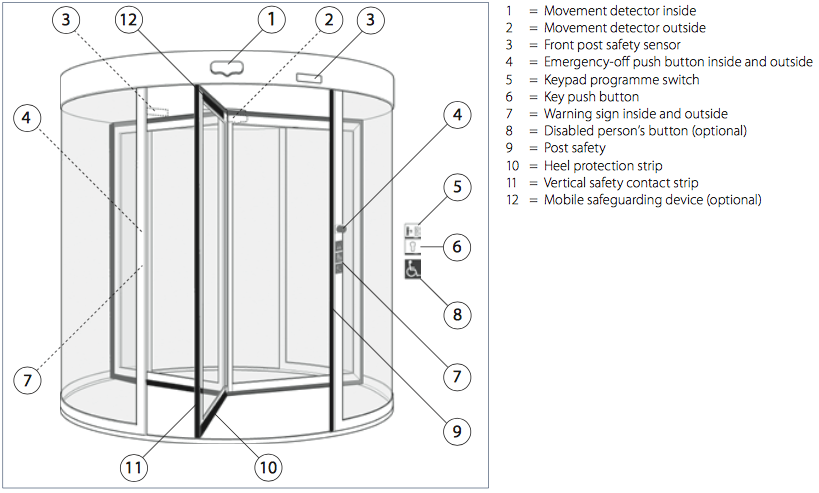
\includegraphics[width=13cm]{./images/Facade/scheme}
\caption{Revolving door selected for terminal building main entrances and exits.}
\end{figure}

For illustration purposes, the result of using these revolving doors in the terminal building would be:

		\begin{figure}[ht!]
	\centering
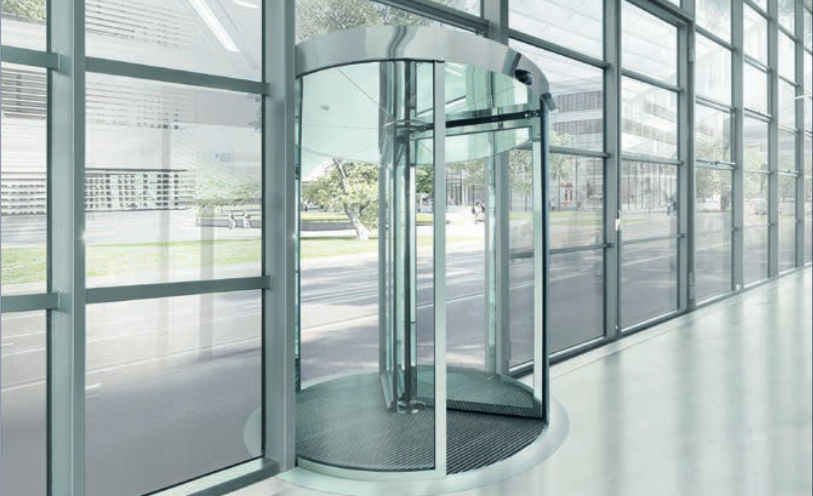
\includegraphics[width=13cm]{./images/Facade/revolving}
\caption{Revolving door selected for terminal building main entrances and exits.}
\end{figure}
	
	
		\subsection{Access bridges}
	Access bridges between terminal and jetway (gangway to the aircraft) are the connecting structures between the jetways to access the aircraft and the terminal building. Due to the dock structure of our terminal, an access bridge will be located at each boarding gate.
	
	The constructive materials in the terminal building are mainly composed of steel beams, the bridge pillars will be made of prefabricated concrete, with the objective of easen the assembly and possible disassembly, in the eventual case that a fixing or a terminal building enlargement are needed.
	
			\begin{figure}[ht!]
	\centering
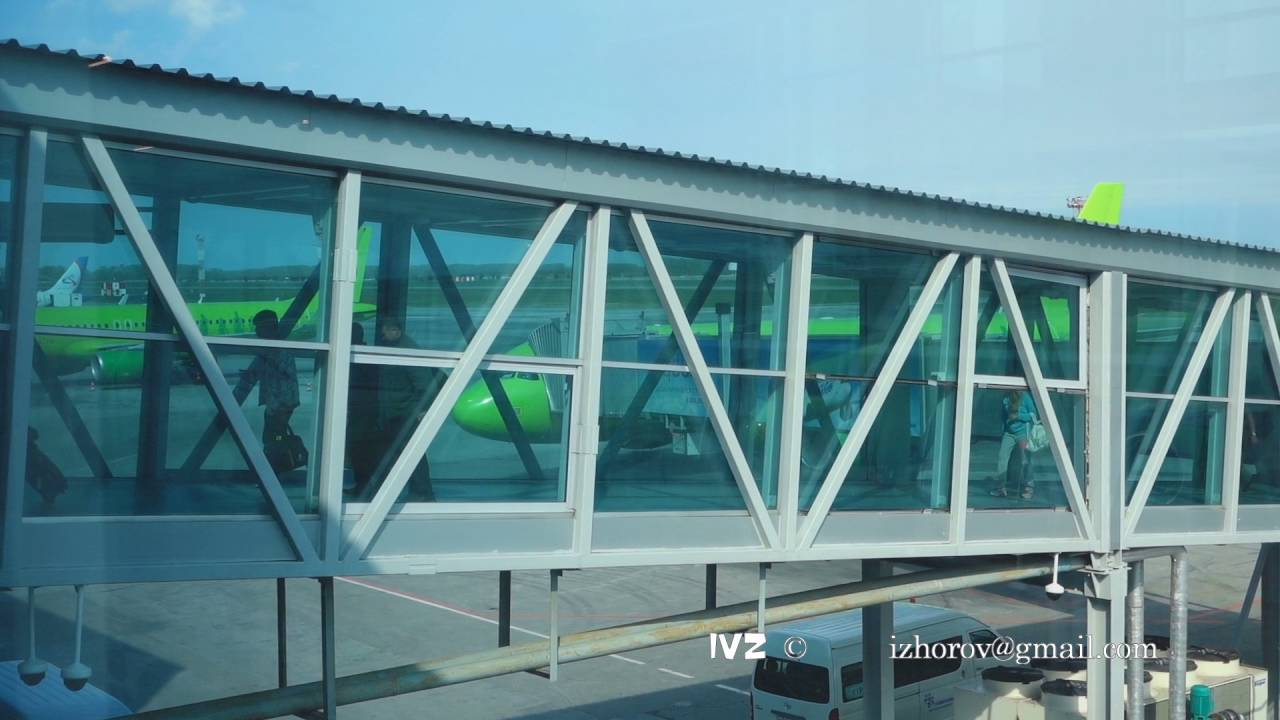
\includegraphics[width=13cm]{./images/Facade/access}
\caption{Access bridge connecting terminal and jetway.}
\end{figure}
	
	For the main bridge structure, steel alloys will be used for ceiling and floor, square shaped profile for vertical bars. Also, transversal beams of cylindrical profile will be used for tangential efforts absorption. 
	
	Asthetical finishings will be done keeping the facade aesthetics followed in the whole terminal building, for that reason the glass will use the same Spider system as presented before in section 5.1.
	
		\subsection{Emergency doors}
	Emergency doors have been subcontracted to the DORMA company. This company offers products for emergencies and escape route systems. 
	
	It has been chosen to use DORMA TV100 doors that are provided with locking devices that immediately unlock secured escape route doors on activation of the emergency pushbutton, in the event of an emergency and for authorized users. 
	
	They are equipped with an electromechanical locking mechanism and provide jam-free unlocking irrespective of loads. Doors are provided with an anti-corrosion protection, since they are made of a very sturdy metal. Furthermore, this system complies with the German guidelines on electrical locking systems for doors used in emergency exits and escape routes (EItVTR).
	
		\begin{figure}[ht!]
	\centering
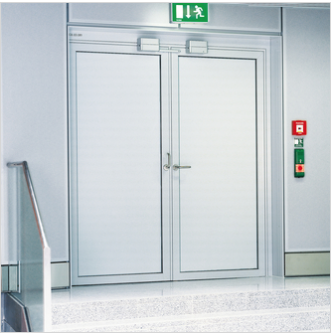
\includegraphics[width=9cm]{./images/Facade/emergencydoor}
\caption{Emergency doors provided by DORMA.}
\end{figure}
		\subsection{Automatic baggage handling system doors}
	ABHS (SATE) access from apron and vice versa, has been decided to be made with a series of doors distributed by all around the building, with the purpose of promoting the efficiency and quickness in loading and unloading baggage. These doors would be roll-up doors, since this way, the door can remain open without disturbing the operators, and be closed when activity is finished. As a consequence, the indoor temperature and humidity can be kept; therefore, reducing heating consumption inside of the building.
	
	The doors chosen have been from the company Stormtite, and the model is AP Model 627. These doors answer the demand for reliability, durability, flexibility and thermal efficiency. 
	
			\begin{figure}[ht!]
	\centering
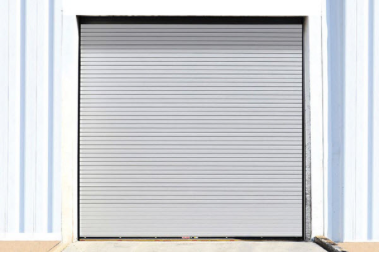
\includegraphics[width=9cm]{./images/Facade/sate}
\caption{Stormtite AP Model 627 doors for ABHS (SATE).}
\end{figure}
	
	
